\documentclass[12pt]{article}

% Packages for formatting
\usepackage{geometry} % 1-inch margins
\geometry{a4paper, margin=1in}
\usepackage{times} % Times New Roman font
\usepackage{setspace} % For double spacing
\usepackage{csquotes}       % For proper quotation formatting \enquote{}
\usepackage{fancyhdr} % For headers and footers
\usepackage{titlesec} % For section numbering
\usepackage{booktabs} % For professional-looking tables
\usepackage{bookmark}
\usepackage[polish,spanish,english]{babel}
\hypersetup{
    colorlinks=true,
    linkcolor=black,
    urlcolor=black,
    citecolor=black
}
\usepackage{graphicx}
\graphicspath{ {./figures/} }
\usepackage[style=apa, backend=biber, language=english]{biblatex} % APA 7th edition references
\usepackage[T1]{fontenc}
\usepackage{caption}
\captionsetup[table]{font=small, labelsep= period, width=0.8\textwidth}
\captionsetup[figure]{font=small, labelsep= period, width=0.8\textwidth} % Options: tiny, scriptsize, footnotesize, small, normalsize, large, Large, etc.
\usepackage{subcaption}

\addbibresource{bibl.bib} % Reference file

% Set double spacing
\doublespacing

% Indent paragraphs by 0.5 inch
\setlength{\parindent}{0.5in}

% Page numbering setup
\pagestyle{fancy}
\fancyhf{}
\rfoot{\thepage} % Page number in the bottom-right corner
\renewcommand{\headrulewidth}{0pt} % Remove the header rule

% Section formatting
\titleformat{\section}[block]{\normalfont\Large\bfseries}{\thesection.}{0.5em}{}

\begin{document}
\pagenumbering{roman}
\section*{Abstract} % maximum 150 words
This project investigates to what extent morphological inflection can be automatically distinguished from derivation based solely on word forms. The debate on inflection and derivation remains highly contentious in linguistic literature, with some viewing them as fundamentally similar or existing on a gradient, while others argue for a clear distinction. Despite extensive theoretical discussions, empirical evidence remains limited. One proposed distinction is semantic regularity: inflection is expected to be stable in its syntactic and semantic effects across lexemes (e.g., cinema is to cinemas as cat is to cats), whereas derivation is less so (e.g., delegation is not to delegate as election is to elect). However, this criterion has yet to be systematically tested large scale cross-linguistically. 
Building on previous work (e.g., \textcite{bonami2018InflectionVsDerivation}; \textcite{rosa2019AttemptingSeparateInflection}), this project uses distributional semantics and word embeddings to assess semantic regularity as a potential proxy for differentiating inflection and derivation. It focuses on two morphologically rich languages, Spanish and Polish. Additionally, the project examines differences in semantic regularity also among various types of inflection, such as case, number, gender, and person.

\section*{Keywords} % maximum 10 keywords
morphology, inflection, derivation

\newpage
\tableofcontents % índice
\newpage

\pagenumbering{arabic} % Switch to Arabic numerals for the main content

\section{Índice provisional}

\begin{enumerate}
    \item Introduction
    \subitem Distinction between inf/der (1 pag? media?)
    \subitem Distributional semantics (media pagina)
    \subitem Word vectors (media pagina)
    \subitem UniMorph (media pagina)
    \subitem Why Polish and Spanish? :D
    \item Methodology 
\end{enumerate}

\newpage
\section{Introduction}
The distinction between morphological inflection and morphological derivation is still an unresolved question. In order to tell them apart, authors provide different criteria (see for instance \textcite{booij2006InflectionDerivation}, \textcite{aronoff2011WhatMorphology}, \textcite{booij2012GrammarWordsIntroduction}, \textcite{haspelmath2013UnderstandingMorphology}, \textcite{stump2005WordFormationInflectionalMorphology} or \textcite{stump2017Inflection}, among many others). Some authors are of the opinion that they are essentially the same thing \parencite{haspelmath2024InflectionDerivationTraditional} or at least that they exist on different ends of a scale or gradient (see \textcite{bybee1985MorphologyStudyRelation} or \textcite{stekauer2015DelimitationDerivationInflection}). Even \textcite{haspelmath2013UnderstandingMorphology} argue that if all criteria are given the same importance then a continuum is the best explanation, since we cannot draw a sharp boundary between both processes. In fact, the same authors often provide examples of exceptions to the very same criteria, so there is no infallible one.

% examples of criteria?

Among the long list of criteria there is one that has been used before in research articles in order to provide empirical results on the distinction debate, there is the semantic regularity criterion: \enquote{Inflection is semantically more regular than derivation.} \parencite{stump2005WordFormationInflectionalMorphology}. Regarding these academic articles that have explored this debate before there is \textcite{bonami2018InflectionVsDerivation}, \textcite{rosa2019AttemptingSeparateInflection} and \textcite{haley2024CorpusbasedMeasuresDiscriminate}, which follow the same criterion even though they take different metrics.

In order to automatically test whether this criterium holds or not, we need to make use of the distributional hypothesis which can be explained as similar words appear in similar contexts. 

% To further explain this criterium it is also said that derivation creates new lexemes whereas inflection creates wordforms (WHAT IS A WORDFORM?) of the same lexeme, both generally using affixes. A lexeme is an abstract word that represents wordforms, that is wordforms such as \textit{eats}, \textit{ate}, \textit{eaten} all relate to a single abstract representation \textsc{eat} (written by convention in small capital letters). In other words, derivation is a lexicon enriching morphological process whereas inflection is a cell filling process.

\section{Background and rationale}

\subsection{Inflection and derivation}

\subsection{Distributional semantics}

\subsection{Word vectors}

\subsection{UniMorph}

\subsection{Related studies}

\section{Methodology}

This study explores the distinction between inflection and derivation in Polish and Spanish using various word embedding models, both static and contextual.

To achieve this, several models were implemented. For static embeddings, used Word2Vec and FastText were used, and for contextual embeddings, the Multilingual BERT model was used. The Word2Vec model for Spanish was trained on the Spanish Billion Words (SBW) corpus. For Polish, the IPIPAN Word2Vec model (nkjp+wiki-forms-all-300-skipg-ns) was used, which is comparable in quality to SBW. It was trained on the National Corpus of Polish (NKJP) and Wikipedia, includes all parts of speech and word forms, and produces 300-dimensional vectors using the skip-gram algorithm with negative sampling. In addition, FastText embeddings for both Spanish and Polish were applied to incorporate subword-level information.

In order to conduct an initial analysis two separate datasets were constructed, one for inflection and another one for derivation, extracting the data from UniMorph.
For the inflection analysis, a Pivot/Inflection dataset was constructed.

The data was filtered to include the following verb tenses in Spanish:
\begin{itemize}
    \item Present Indicative. UniMorph category: V;IND;PRS.
    \item Past Imperfect. UniMorph category: V;IND;PST;IPFV.
    \item Future Indicative. UniMorph category: V;IND;FUT.
\end{itemize}


This resulted in a dataset of 148,051 rows, each consisting of a base form, its inflected form, and the morphological category. Additional forms such as participles and gerunds are planned for future inclusion.

 In Polish the filtering included:
\begin{itemize}
    \item Present. UniMorph category: V;PRS.
    \item Past. UniMorph category:V;PST.
    \item Future. UniMorph category:V;FUT.
\end{itemize}

The resulting dataset contains 23,615 rows. For the derivation analysis the data provided by UniMorph was used without changes.

% ejemplo de dataset aqui

The initial analysis revealed some errors in both datasets. In the derivations dataset the label U (unspecified or unknown) presented some issues. The goal is to eliminate all instances of unknown categories, to get rid of this noise and have cleaner results and means.

1. In Spanish there are 20 rows that contain a derivation that results in U (i.e. N:U or V:U) and 107 in Polish. 
2. On the other hand, there are even more derivations in which the pivot is tagged with U (U:N, U:ADJ...), 36 in Spanish and 253 in Polish. 

\subsection{Cleaning the derivational dataset}

Taking a quick look through this data one can see many mistakes such as formatting issues or  verbs, adjectives or nouns being labeled U. When it comes to Spanish, the number is not too high, so it is something that is worth fixing in order to get rid of this label. Fixing the first group seems fairly easy since a category can be assigned based on the affix.

In order to clean the Spanish derivations dataset a new category according to the affix was assigned. All the affixes that end in *-ero*, *-ez*, *-ismo*,*-í* and *-illa* were changed to N. V was also assigned to those that contain the affixes *-ar* and *-ear*. As a result 6 rows were obtained. They can be eliminated from the final dataset because of all the mistakes they contain.

The second group of Spanish derivations (:U) cannot be easily fixed with a Python script, it contains many numerals and words that are not N, ADJ, ADV or V. Those rows that do not contain any of such categories can be dropped and the rest probably needs to be fixed manually. It contais some verbs, nouns and adjectives labeled with U, for instance *cuarenta cuanrentóń U:N -ón*. For some reason *cuarenta* is labeled in other rows as N but not in this one. Since numerals can be N or ADJ, alongside all the other issues with this group all these rows (35) can be dropped. It is a low number that will not affect the results.

Polish data seems to need more work as there are more incorrect labels, but it can be fixed more easily. Affixes such as *-any*, *-ony*, *-ty*, *-y*, or *-ący*, *-ęty* take the label ADJ, because they are all endings that participles take. There also are some formatting issues. Some rows under the same condition (X:U) contain the pivot and the derived form joined together in the pivot cell (i.e. *mylićpomylić	pomylić*). This can be fixed as well just removing the form from the pivot column and assigning to row the correct categories. Some rows that contained verbs in both columns but were not correctly labeled, so they were fixed as well. This was fairly easy since in Polish verbs in the infinitive form end in *-ć* (most of them) or *-c*. Three rows incorrectly labeled U:U were changed to ADJ:ADJ since they contained adjectives.

The table above represents the rest, which can be removed as well as they do not contain any nouns, adjectives, adverbs or verbs. Take for instance the appearance of *co*, *kto* or *jaki*. which are relative pronouns. Everything ending in *-ś* and *-ż* or *-że* are not nouns nor adjectives nor adverbs nor verbs, but other types of pronouns or particles, so they can be removed. Regarding the data labeled as U:X, it can be done much better than in Spanish because there are many rows (163) that contain verbs ending in *-ć* in both the pivot and the derivation column but are incorrectly labeled as U:V, for example *kręcić skręcic U:V s-* or *paść przepaść U:V prze-*. The label change to V:V can easily be done. There are also 27 rows that contain verbs ending in *-c* in both the pivot and the derivation cells, which can be fixed just like previously done on the other group of verbs.

Finally some pivots that are verbs but are not labeled as such can be changed just by looking at the ending, although this needs to be done carefully as some nouns can also end in *-ć* or *-c*, for this reason it will only be done on the mislabeled ones (the ones labelled as U), which are all verbs.

Since almost 200 rows have been fixed, the resulting ones labeled as U:X contain only 21 rows, with some mistakes or words that are not N, ADJ, ADV or V so they can just be dropped. Both resulting datasets do not contain any row labeled with U anymore.

\begin{table}[ht]
\centering
\label{tbl:mean-similarity}
\begin{minipage}[t]{0.48\textwidth}
\small
\centering
\subcaption*{Inflection}
\begin{tabular}{llc}
\toprule
\textbf{Model} & \textbf{Language} & \textbf{Mean Similarity} \\
\midrule
\textbf{FastText}  & Spanish & 0.51 \\
                   & Polish  & 0.54 \\
\textbf{Word2Vec}  & Spanish & 0.50 \\
                   & Polish  & 0.40 \\
\textbf{Mult BERT} & Spanish & 0.92 \\
                   & Polish  & 0.93 \\
\bottomrule
\end{tabular}
\end{minipage}
\hfill
\begin{minipage}[t]{0.48\textwidth}
\small
\centering
\subcaption*{Derivation}
\begin{tabular}{llc}
\toprule
\textbf{Model} & \textbf{Language} & \textbf{Mean Similarity} \\
\midrule
\textbf{FastText}  & Spanish & 0.51 \\
                   & Polish  & 0.54 \\
\textbf{Word2Vec}  & Spanish & 0.50 \\
                   & Polish  & 0.40 \\
\textbf{Mult BERT} & Spanish & 0.92 \\
                   & Polish  & 0.93 \\
\bottomrule
\end{tabular}
\end{minipage}
\caption{Mean similarity between pivot and form in inflection and derivation by model and language}
\end{table}


\subsection{Cleaning the inflectional dataset}

The only thing to clean in the inflections dataset are the *vos* and *usted* forms.

\subsection{Subsetting the most frequent lemmas and affixes}

For this task in Spanish the 10000 most frequent lemmas in CREA was used. The verbs that appear in both datasets, UniMorph and CREA, were extracted and a subset of 1568 lemmas was obtained from a total of 6695. 

For the Polish data sgjp.pl was used. Using the site's implemented filter the 8500 most common lexemes were extracted and after filtering the verbs from that list, 1832 verbs were obtained. Afterwards that list of verbs was compared to the UniMorph data and  those that appear in both datasets were extracted resulting in 455 lemmas from a total of 844 that appear in the UniMorph data.

To create the subset of affixes, the most common affixes in the UniMorph data itself were taken.

\begin{table}[ht]
\centering
\label{tbl:affixes}
\begin{minipage}[t]{0.48\textwidth}
\centering
\subcaption*{Spanish}
\begin{tabular}{lr}
\toprule
\textbf{Affix} & \textbf{Count} \\
\midrule
-mente  & 2997 \\
-dor    & 1316 \\
-ar     & 1310 \\
-ero    & 1123 \\
-miento & 913  \\
-ico    & 870  \\
des-    & 836  \\
-ción   & 831  \\
-ear    & 676  \\
-ista   & 642  \\
-ito    & 638  \\
-ismo   & 549  \\
-ón     & 533  \\
-idad   & 499  \\
-al     & 491  \\
\bottomrule
\end{tabular}
\end{minipage}
\hfill
\begin{minipage}[t]{0.48\textwidth}
\centering
\subcaption*{Polish}
\begin{tabular}{lr}
\toprule
\textbf{Affix} & \textbf{Count} \\
\midrule
-owy   & 5804 \\
-ka    & 5487 \\
-anie  & 3421 \\
-ość  & 3287 \\
-ny    & 2414 \\
-ie    & 2161 \\
-enie  & 1669 \\
-ek    & 1521 \\
-ować  & 1517 \\
-o     & 1393 \\
-ik    & 1249 \\
-ski   & 1212 \\
-ąć   & 1158 \\
-stwo  & 770  \\
za-    & 742  \\
\bottomrule
\end{tabular}
\end{minipage}
\caption{Top 15 affixes in Spanish and Polish in UniMorph data.}
\end{table}

\begin{table}[ht]
\centering
\label{tbl:subset-results}
\begin{minipage}[t]{0.48\textwidth}
\small
\centering
\subcaption*{Inflection}
\begin{tabular}{llc}
\toprule
\textbf{Model} & \textbf{Language} & \textbf{Mean Similarity} \\
\midrule
\textbf{FastText}  & Spanish & 0.49 \\
                   & Polish  & 0.49 \\
\textbf{Word2Vec}  & Spanish & 0.50 \\
                   & Polish  & 0.53 \\
\textbf{Mult BERT} & Spanish & 0.93 \\
                   & Polish  & 0.90 \\
\bottomrule
\end{tabular}
\end{minipage}
\hfill
\begin{minipage}[t]{0.48\textwidth}
\small
\centering
\subcaption*{Derivation}
\begin{tabular}{llc}
\toprule
\textbf{Model} & \textbf{Language} & \textbf{Mean Similarity} \\
\midrule
\textbf{FastText}  & Spanish & 0.51 \\
                   & Polish  & 0.54 \\
\textbf{Word2Vec}  & Spanish & 0.50 \\
                   & Polish  & 0.40 \\
\textbf{Mult BERT} & Spanish & 0.92 \\
                   & Polish  & 0.93 \\
\bottomrule
\end{tabular}
\end{minipage}
\caption{Mean similarity between pivot and form in inflection and derivation by model and language on the subset data.}
\end{table}


\begin{figure}[ht]
\centering
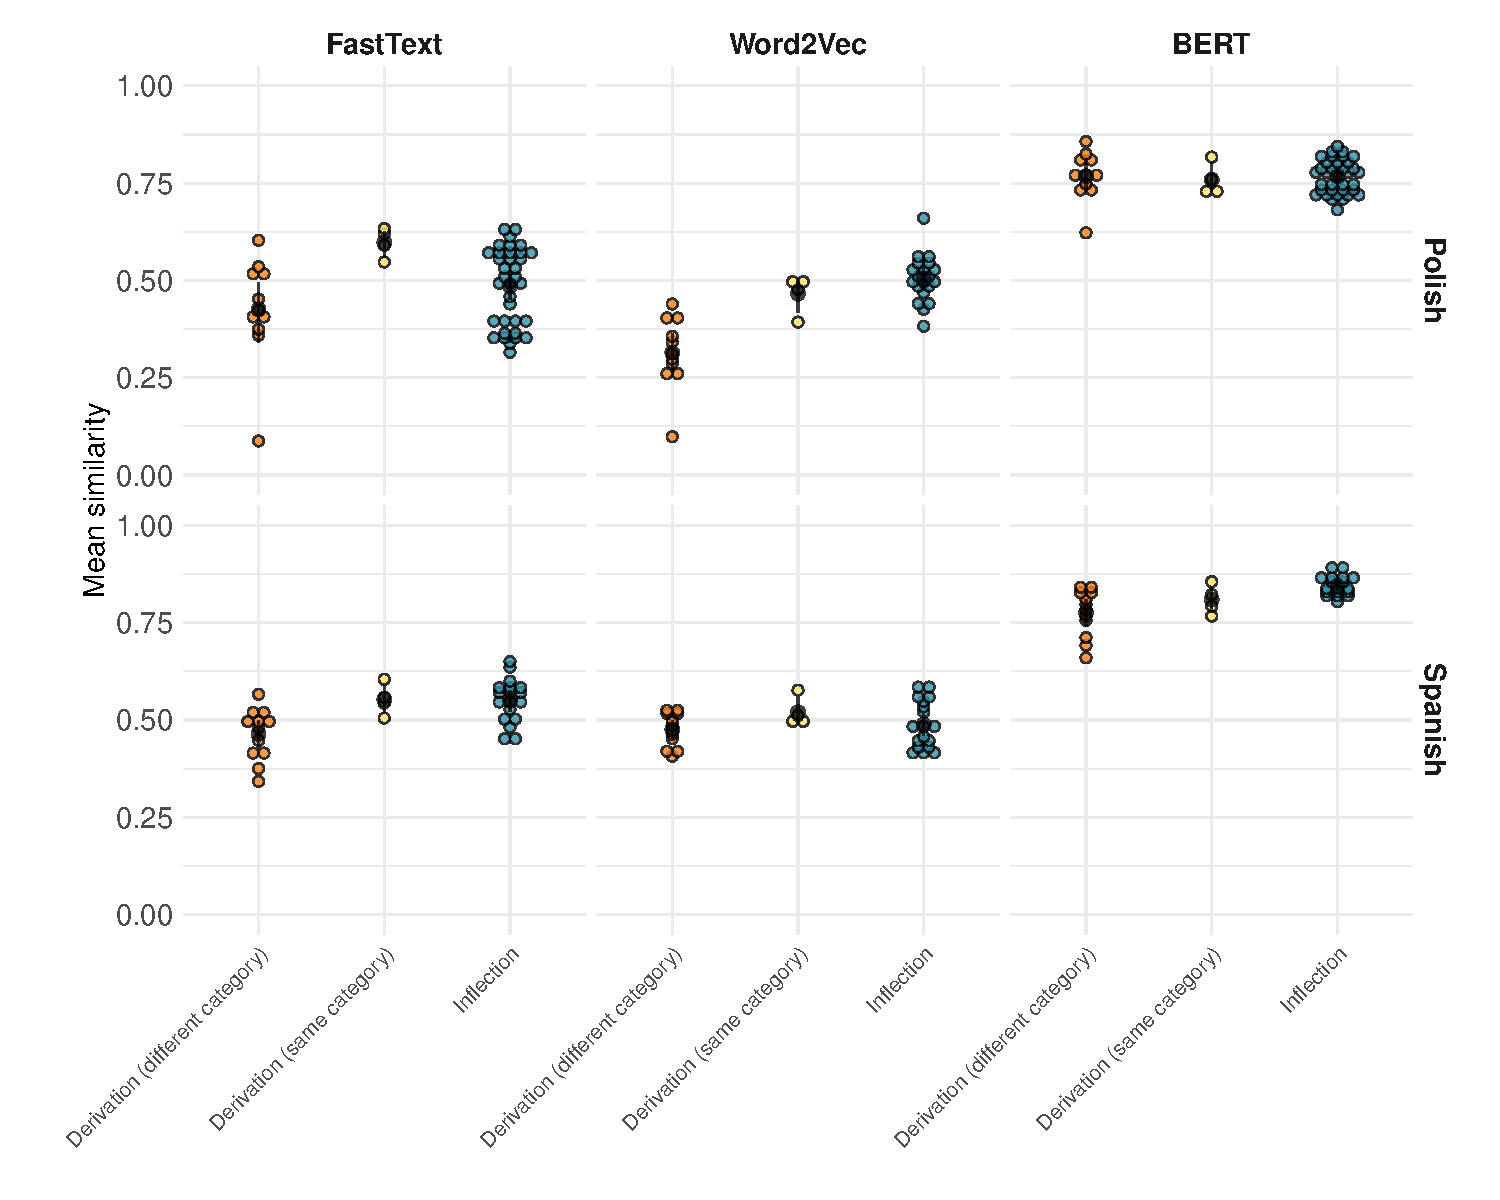
\includegraphics[width=\textwidth]{fig-clean.pdf}
\caption{Mean similarity between pivot and form in inflection and derivation by model and language.}
\label{fig:clean-data}
\end{figure}

% shuffled data plot, subset data plot

\subsection{Implementing a random baseline}
The previous baseline shuffled the whole data 10 times. In this case a better baseline is implemented. It consists of filtering the data, that is separately filtering inflections by tense (present, past or future) and derivations by category, then shuffling each filter 100 times while extracting the mean similarity of the whole filtered data. That means we are extracting the mean similarity a hundred times by type of morphological process (inflection or derivation), tense/category, model and language and plotting its distribution.

\begin{figure}[p]
\centering
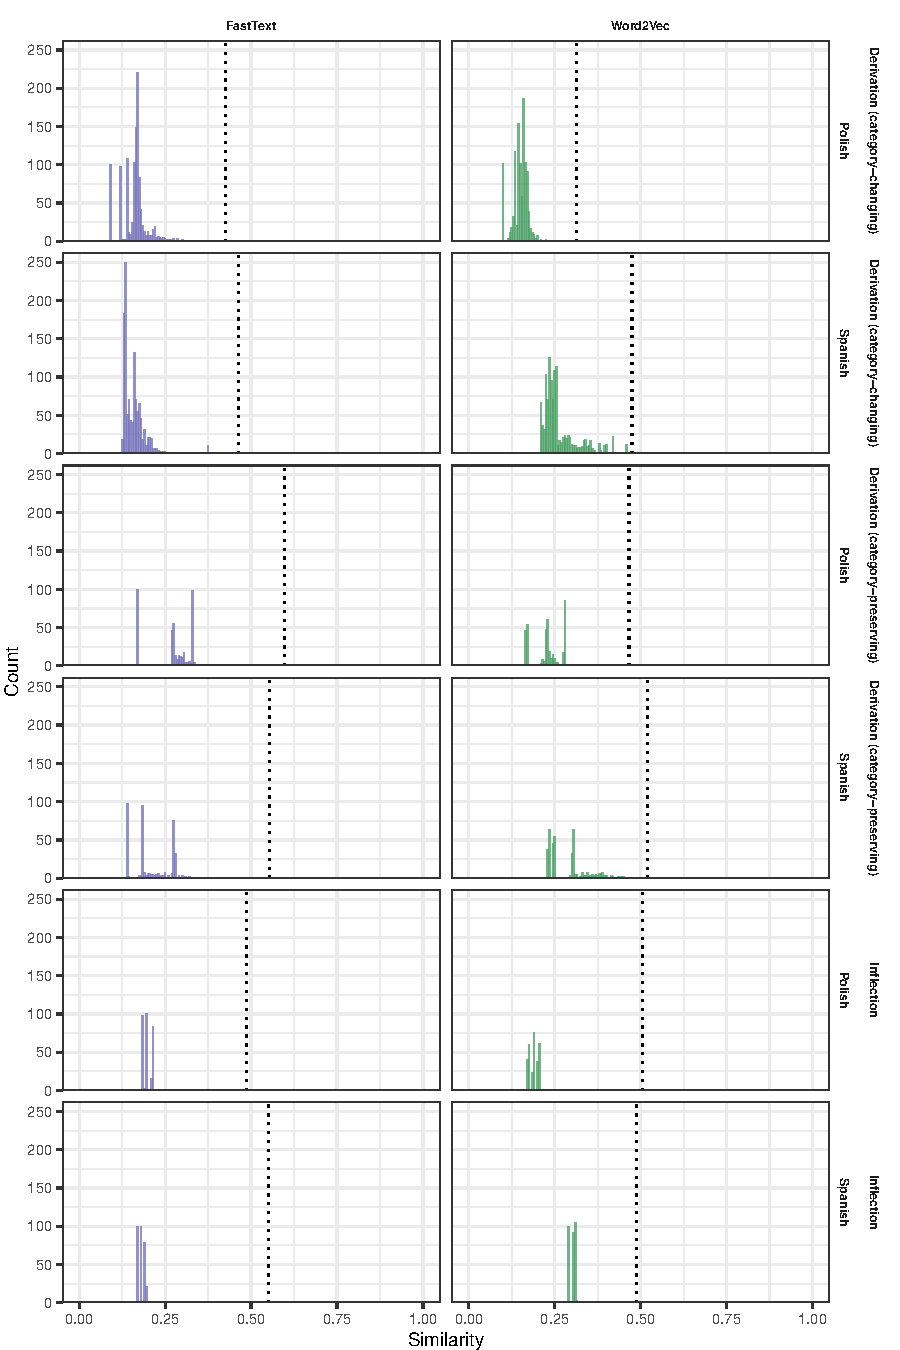
\includegraphics[height=0.95\textheight,width=\textwidth]{fig-baseline-faceted.pdf}
\caption{Random baseline}
\label{fig:baseline}
\end{figure}

\section{Conclusion}

% Print bibliography
\newpage
\addcontentsline{toc}{section}{References}
\sloppy
\printbibliography

\end{document}
